%----------------------------------------
% Write your notes here
%----------------------------------------


\section{Outline}

\begin{itemize}
  \item Classification
  \item Logistic Regression, with examples in R \\
  Vowpal Rabbit Example
  \item Networks \\
  History\\
  Structures and Applications
\end{itemize}


\section{Classification}
Question: why not solve Classification as a regression problem?\\

More precisely, say you have a set of response y variables that take values of either 0 or 1, and a set of x values that take any values on the real line.
\begin{eqnarray*}
  x \in \mathbf{R} \\
  y \in \{0, 1\}
\end{eqnarray*}

Why not model a linear regression solution using OLS? That is, fit a model like:

\begin{eqnarray*}
  \hat{y} = w \cdot x \\
  \textrm{ where }
  w = \frac{ \mathbf{x} \cdot \mathbf{y} }{\mathbf{x} \cdot \mathbf{x}} \\
  \textrm{, minmizing the loss function: }\\
  L = \frac{1}{n} \sum_i \big(y_i - \hat{y_i}\big)^2
\end{eqnarray*}

Look at the example plot (on the next page)

\begin{figure}[ht]
  \begin{center}
    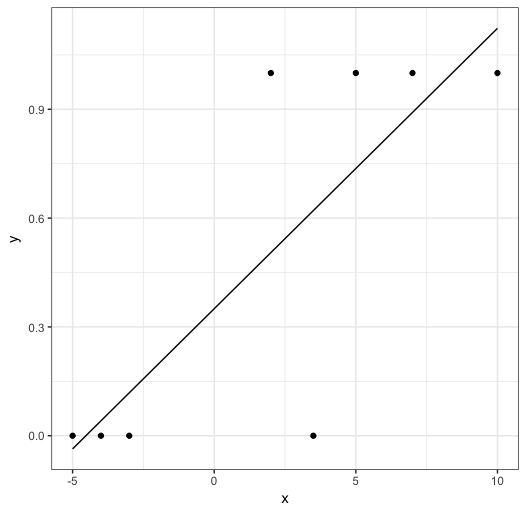
\includegraphics[width=0.5\textwidth]{figures/CAR.png}
    \label{fig:Solving Classification using Linear Reggredssion}
  \end{center}
\end{figure}



We can see that the point at the top right is giving a non zero loss, even though the line is above 1, and so it would predict the right label, but would still give some loss. 

One possible fix to this, that is used in practice, is to set up a piece-wise linear model that is 1 if the prediction is greater than 1, and zero if the prediction in less that zero. 
\begin{eqnarray*}
  \hat{y} = 1 \textrm{ if } w\cdot x > 1 \\
      0 \textrm{ if } w\cdot x < 0 \\
      w\cdot x \textrm{ otherwise}
\end{eqnarray*}

Sort of like a piece-wise-linear, jagged version of logistic Regression

\section{Logistic Regression}
Review: the model make a linear fit to the log odds:

\begin{eqnarray*}
  \ln (\frac{p}{1-p}) = w\cdot x \\
  \textrm{This minimizes the loss function:}\\
  L = \prod_i p_i^{y_i}\cdot(1-p_i)^{1-y_i}
\end{eqnarray*}

We then went through an example analyzing the chances of survival for passengers on the Titanic. (See class github page for the R file). The main takeaways are:
\begin{itemize}
  \item Coefficients returned from logistic regression models can be difficult to interpret, as they relate to log-odds, although it is possible to make the tranformations to regular probabilities
  \item Instead, it can be much easier to analyze predictions against observations
  \item As more variables are added into the model, the results are harder to interpret
\end{itemize}

Next, we looked at machine-learning based models:
\begin{itemize}
  \item goals are less about model interpretability
  \item prioritizes ability fro large-scale data processiong
  \item solely for prediction, quickly
\end{itemize}

One such machine-learning based approach we looked at was Vowpal Rabbit, which has the following advantages:
\begin{itemize}
  \item Input formal is very easy, fast (Uses Stochastic Gradient Descent)
  \item Speed is fast
  \item It is scalale, can deal with a large number of features
  \item Feature pairing, progressive validation
  \item can do logistic regression, but can also do much more!
\end{itemize}



\section{Networks}
In our previous models, there has been an assumption of independence between datapoints. With networks, this assumption does not hold, and instead the datapoints are relational. Networks have both mathematical and social applications. First, a brief look at the history of Networks:
\begin{itemize}
  \item first looked at Granoveter paper, modeling two individuals' number of mutual friends as a function of the strength of their frienship. (stronger friendship = more mutual friends)
  \item analyzing the success of academic papers. We could see the "long tail" that we've discussed in previous classes... most papers don't get cited much, if at all. 
  \item Next, we looked at Watts and Strogat's Small-World Networks. A regular network sees no random connections between nodes, and a random network has only random connections between nodes. A small-world network is somewhere in between, with some randonm connections and some nonrandom connections. This model has the ability to capture long-ranging ties, i.e. the "6 degrees of separation" phenomenon. 
  \item we saw another plot illustration the connections that blogs have. The plot observed a disconnect between different sides of the political spectrum.
\end{itemize}

Next, we Looked at types of Networks. There can be many applications for networks, such as modeling social, info, activity, biological or geographical networks. There is no single way to represent networks, but there are usually connections illustrated between nodes. Features of networks can also be directed, weighted...

There are many ways to store network data. Here are a few examples (see the lecture notes for graph visualizations):
\begin{enumerate}
  \item Edge List \\
    \begin{itemize}
      \item Is a list made up of every edge, with each entry containing the two nodes the edges connects
      \item simple storage
      \item bad for computation, computational complexity is O(number of edges)
    \end{itemize}
  \item Adjacency Matrix
    \begin{itemize}
       \item a square matrix, where each row and column index is a node
       \item grid of 1's and 0's. 1 represents a connection between nodes, 0 means no connection
       \item this is quick to check edges
       \item good for linear algebra
       \item matrix is often sparse
      \end{itemize}
  \item Adjacency List
   \begin{itemize}
        \item for each node, there is a list of what other node is connected to
        \item this is good for graph traversal
        \item if directed graph, needs 2 lists per node
      \end{itemize}
\end{enumerate}


There are many features that can be used to desctibe networks:
\begin{itemize}
  \item degree - number of connections a node has
  \item path lenght - shortest past between nodes
  \item clustering
  \item components - how many disconnected parts does the network have?
\end{itemize}











